%%%%%%%%%%%%%%%%%%%%%%%%%%%%%%%%%%%%%%%%%%%%%%%%%%%%%%%%%%%%
%
% Authors:       Nina Wiedemann, Benjamin Ummenhofer, Diana Wofk, 
%                Quentin Leboutet, and Michael Paulitsch
%
% Description:   The SYCL of Life: Evolutionary Kernel Optimization 
%                with Large Language Models
%
% Section:       Results
%
%%%%%%%%%%%%%%%%%%%%%%%%%%%%%%%%%%%%%%%%%%%%%%%%%%%%%%%%%%%%

\section{Experimental setup}\label{sec:experiments}

The field of kernel generation faces challenges in making fair comparisons, because results depend heavily on the hardware used, the programming approach, and the abilities of the LLM. To address this, we carefully control these factors and conduct experiments across several benchmarks, using different hardware types and programming languages. 


\paragraph{Programming paradigm and hardware.} 
KernelFoundry supports CUDA, SYCL, and Triton. Our primary focus is on SYCL for Intel hardware. SYCL offers several advantages: (1)~it is an open industry standard (Khronos Group) rather than a proprietary language; (2)~it provides C++ abstractions that 
are more amenable to LLM generation than low-level intrinsics; (3)~it enables true cross-platform portability with a single codebase. The experiments are conducted on an integrated Intel Arc 140V GPU and a discrete Intel Battlemage B580 GPU, as well as an NVIDIA RTX A6000 GPU with Ampere architecture (for CUDA comparisons). We implement a rigorous kernel performance benchmarking with several improvements over prior work (see \autoref{app:implementation}).


\paragraph{Benchmarks.}\label{sec:experimental_benchmarks}
We evaluate on  \textit{KernelBench}~\citep{ouyang2025kernelbench} as the de-facto standard for LLM kernel generation, comprising 250 tasks across three levels (L1: single operators, L2: fusion patterns, L3: full architectures). Following~\citet{lange2025towards} and \citet{metr}, we filter out flawed tasks prone to reward hacking or with inefficient baselines, resulting in a filtered set of 111 tasks (80 L1, 31 L2). For most experiments, we use a representative subset of 40 tasks (20 L1, 20 L2), that is selected based on related work (see Appendix~\ref{app:kernelbench_filtering}).
Secondly, we utilize 12 tasks from \textit{Robust-kbench}~\citep{lange2025towards}. They provide 19 tasks including forward-backward operations; however, they published their results (i.e., the best generated kernel, required for comparison) only for 12 of those.


\paragraph{Baselines.}
Unfortunately, most related works only publish aggregated numbers such as the average speedup per level, usually across all KernelBench problems, and not the generated kernels themselves. Since some KernelBench tasks are flawed and allow reward hacking, and the performance is highly hardware dependent, comparability to these results is inhibited. We thus compare to prior work that publish their best-performing kernels: robust\_kbench~\cite{lange2025towards}, the AI CUDA Engineer~\cite{lange2025ai} and Kernelsseum~\cite{kernelsseum, ouyang2025kernelbench}. 
Due to model deprecation and access restrictions, we are limited to using only the available subset of the LLMs used in the baselines, which presents additional challenges for our method. % (see \autoref{tab:baseline_comparison})
For comparison with robust-kbench, we utilize GPT-\{o3,o4-mini,4.1\}, excluding Sonnet 3.7 used in their method. For comparing to the AI CUDA engineer we could only use o3-mini (excluding DeepSeek-\{v3,R1\}, GPT-\{o1-preview,o1-high\}, and Sonnet 3.5). 
Further hyperparameter settings are given in Appendix~\ref{app:implementation}.


\paragraph{Metrics.}
Following prior work, we report the correctness rate (fraction of tasks with a kernel that compiles and yields numerically correct outputs) and the fast$_p$ metric, defined as the proportion of tasks with a speedup greater than p: $\frac{1}{N} \sum_{i=1}^N \mathbf{1}[\text{speedup}_i > p]$ where $N$ is the number of tasks, and the speedup is the baseline time (pytorch eager execution if not denoted otherwise) divided by the kernel execution time. 
For correctness, we apply stricter criteria than prior work since we noticed that the precision used by KernelBench is very low, in particular the absolute precision of $10^{-2}$, allowing erroneous kernels to pass in cases of small output values which commonly appear with AI operations. We thus rely on the relative precision $\nu = \frac{| y - \hat{y}|}{|y| + \epsilon}$, where $y$ is the expected output, $\hat{y}$ is the kernel output, and $\epsilon$ is a small value preventing division by zero. However, due to hardware imprecision, errors should be allowed in a small fraction of cases. Thus, we define a kernel as correct if $\nu < 0.01$ in 99\% of the output values. As a second measure for kernel correctness, we propose the cosine similarity of the flattened output tensors as a measure of their angular divergence.


\section{Results} \label{sec:results}

We first evaluate KernelFoundry's ability to generate CUDA kernels in comparison to prior work, and then demonstrate its versatility by generating SYCL kernels. Furthermore, we showcase its adaptability to custom tasks and analyze hardware-specific aspects.

\subsection{Baseline comparison}

\autoref{tab:baseline_comparison} compares our method to the kernels published by ``AI CUDA Engineer'' and the robust-kbench method on the respective task set for which the baseline kernels were available. We reproduce the speedup of these kernels on our NVIDIA hardware for fair comparison; original results are listed for reference but are not directly comparable due to hardware-specific PyTorch execution times. We further include the results originally published within KernelBench (``Kernelsseum''). \autoref{tab:baseline_comparison} shows that the kernels generated with our approach consistently outperform the baselines, despite using only a subset of the LLMs. Specifically, our approach leads to an average speedup of 1.24 on the KernelBench subset L1 and 2.1 on L2, compared to 1.01 and 1.61 for the kernels published by~\citet{lange2025ai}. On the 12 robust-kbench tasks which include backward operations, our approach also results in a 36\% higher speedup compared to the best kernels published by \citet{lange2025towards}. 
While for many tasks the general evolutionary selection procedure already finds the suitable parameters (e.g. tile size), our parameter optimization, applied only for 2 iterations (best@8), can push the performance in some cases, leading to a notable improvement. For results on a per-task level, see \autoref{app:pertaskresults}.

\begin{table*}[ht]
    \centering
    \resizebox{\linewidth}{!}{%
    \renewcommand{\theadfont}{\normalfont\bfseries}
\begin{tabular}{lllrrrrr}
\toprule
\thead[l]{Task set\\{}\normalfont$n=\text{count}$} & \textbf{Method} & \thead{LLMs} & \thead[c]{Correct\\ rate} & \textbf{fast}$_1$ & \textbf{fast}$_2$ & \thead[c]{Avg.\\ speedup} & \thead[c]{Geom.\\ speedup} \\
\midrule
% \multicolumn{8}{l}{\textit{Baseline comparison on CUDA (controlled hardware and LLMs)}} \\
% \midrule
\multirow{5}{*}{\rotatebox{0}{\parbox{18mm}{\raggedright KernelBench\\repr.\ set L1 $n=20$}}} 
 & Kernelsseum* &  GPT-\{o1,4o\}, DeepSeek-Coder, Sonnet-3.5, LLama-3.1-405B
 & 0.65 & 15 \% & 0 \% & 0.765 & 0.600 \\
 & AI CUDA Engineer original\textsuperscript{\textdagger} &  DeepSeek-\{v3,R1\}, GPT-\{o1-preview,o1-high,o3-mini\}, Sonnet-3.5 & 1.0 & 70 \% & 20 \% & 1.422 & 1.222 \\
 & AI CUDA Engineer re-eval &  DeepSeek-\{v3,R1\}, GPT-\{o1-preview,o1-high,o3-mini\}, Sonnet-3.5 & 1.0 & 40 \% & 50 \% & 1.005 & 0.909 \\
 & Ours &  o3-mini & 1.0 & \textbf{55 \%} & 10 \% & 1.204 & 1.092 \\
 & Ours + parameter optim. &  o3-mini & 1.0 & \textbf{55 \%} & \textbf{15 \%} & \textbf{1.241} & \textbf{1.124} \\
\midrule
\multirow{5}{*}{\rotatebox{0}{\parbox{18mm}{\raggedright KernelBench\\repr.\ set L2 $n=20$}}}  
 & Kernelsseum* &  GPT-\{o1,4o\}, DeepSeek-Coder, Sonnet-3.5 & 0.65 & 10 \% & 0 \% & 0.874 & 0.854 \\
 & AI CUDA Engineer original\textsuperscript{\textdagger} &  DeepSeek-\{v3,R1\}, GPT-\{o1-preview,o1-high,o3-mini\}, Sonnet-3.5 & 1.0 & 100\% & 10 \% & 1.589 & 1.524 \\
 & AI CUDA Engineer re-eval &  DeepSeek-\{v3,R1\}, GPT-\{o1-preview,o1-high,o3-mini\}, Sonnet-3.5 & 1.0 & 85 \% & 25 \% & 1.606 & 1.515 \\
 & Ours &  o3-mini & 1.0 & \textbf{90 \%} & 40 \% & 2.051 & 1.680 \\
 & Ours + parameter optim. &  o3-mini & 1.0 & \textbf{90 \%} & \textbf{45 \%} & \textbf{2.104} & \textbf{1.730} \\
\midrule
\multirow{4}{*}{\rotatebox{0}{\parbox{17mm}{\raggedright Robust-kbench\\{} $n=12$}}} &
Robust-kbench original\textsuperscript{\textdagger} &  GPT-\{o3,o4-mini,4.1\}, Sonnet-3.7 & 1.0 & 92 \% & 50 \% & 15.622 & 2.591 \\
 & Robust-kbench re-eval &  GPT-\{o3,o4-mini,4.1\}, Sonnet-3.7  & 1.0 & 92 \% & 58 \% & 8.865 & 3.499 \\
 & Ours &  GPT-\{o3,o4-mini,4.1\} & 1.0 & \textbf{100 \%} & \textbf{67 \%} & \textbf{12.107} & \textbf{5.295} \\
 & Ours + parameter optim. &  GPT-\{o3,o4-mini,4.1\} & 1.0 & \textbf{100 \%}  & \textbf{67 \%} & 12.081 & 5.225 \\
\bottomrule
\end{tabular}
}
\caption{Comparison to baselines on CUDA kernel optimization. Best results per task set in bold. *\emph{Kernelsseum} evaluated on Nvidia L40S. \textsuperscript{\textdagger}\emph{AI CUDA Engineer original} and \emph{Robust-kbench original} both evaluated on Nvidia H100. All others evaluated on Nvidia A6000.}
\label{tab:baseline_comparison}
\end{table*}

\begin{table*}[ht]
    \centering
    \resizebox{\linewidth}{!}{%
    \renewcommand{\theadfont}{\normalfont\bfseries}
\begin{tabular}{llllrrrrr}
\toprule
\thead[l]{Task set\\{}\normalfont$n=\text{count}$} & \textbf{Method} & \textbf{Language} & \thead{LLMs} & \thead{Correct\\ rate} & \textbf{fast}$_1$ & \textbf{fast}$_2$ & \thead{Avg.\\ speedup} & \thead{Geom.\\ speedup} \\
% \midrule
% \multicolumn{8}{l}{\textit{Expanding to other languages}} \\ 
% \midrule
% KernelBench all [250] (*) & KernelBench leaderboard & CUDA & 0.62 & 0.21 & 0.04 & 1.00 & 0.68 \\
% KernelBench L1 + L2 [200] (*) & Kevin (**) & CUDA & 0.91 & &  &  1.56 & \\
% \midrule
% KernelBench lenient filter [222] & KernelBench leaderboard & CUDA & 0.60 & 0.19 & 0.03 & 0.94 & 0.63 \\
% KernelBench lenient filter [223] & Ours (best overall) & SYCL & 0.97 & 0.66 & 0.34 & 2.33 & 1.23 \\
% KernelBench lenient filter [179] & Ours (best overall) & CUDA & 0.99 & 0.70 & 0.18 & 1.69 & 1.20 \\
\midrule
% KernelBench filtered [111] & KernelBench leaderboard & CUDA & 0.58 & 0.13 & 0.01 & 0.70 & 0.50 \\
% KernelBench filtered [109] & Ours (best overall) & CUDA & 0.99 & 0.60 & 0.12 & 1.26 & 1.00 \\
\multirow{2}{*}{\rotatebox{0}{\parbox{29mm}{KernelBench \mbox{filtered}\\{} $n=111$}}}
 & Ours & SYCL & GPT-\{4.1, 5-mini\}, Sonnet-4.5 & 0.97 & 71 \%  & 42 \%  & \textbf{2.32} & 1.38 \\
 & Robust-kbench & CUDA & GPT-\{o3, o4-mini, 4.1\}, Sonnet-3.7
 & - & - & - & 1.49 & - \\
\midrule
\multirow{4}{*}{\rotatebox{0}{\parbox{19mm}{\raggedright KernelBench repr.\ set L2 $n=20$}}}
 & OpenEvolve (40 iters) & SYCL & GPT-\{4.1, 5-mini\}, Sonnet-4.5 & 1.0 & 70 \%  & 40 \%  & 2.535 & 1.775 \\
 & Ours (40 iters + param. optim.) & SYCL & GPT-\{4.1, 5-mini\}, Sonnet-4.5 & 1.0 & \textbf{80 \%}  & \textbf{45 \%}  & \textbf{2.732} & \textbf{2.119} \\
 & OpenEvolve (10 iters) & SYCL & GPT-\{4.1, 5-mini\}, Sonnet-4.5 & 1.0 & 70 \%  & 20 \%  & 1.483 & 1.202 \\
 & Ours (10 iters) & SYCL & GPT-\{4.1, 5-mini\}, Sonnet-4.5 & 1.0 & \textbf{80 \%}  & 35 \%  & 2.059 & 1.661 \\
\bottomrule
\end{tabular}
}
\caption{Evaluating KernelFoundry on SYCL kernel generation.}
\label{tab:sycl_results}
% \vspace{-4mm}
\end{table*}

\subsection{Evaluation on SYCL kernel generation}

\autoref{tab:sycl_results} presents our results for SYCL kernel generation. For comparison, we include robust-kbench CUDA performance on the filtered KernelBench tasks, as reported in \cite{lange2025towards}. Although SYCL is less commonly used and less familiar to LLMs than CUDA, our method finds correct kernels in 97\% of cases and achieves an average speedup of 2.32. We further compare to OpenEvolve, the open-source implementation of AlphaEvolve~\cite{novikov2025alphaevolve}, which uses an evolutionary algorithm but lacks kernel-specific optimization strategies, meta-prompting, and parameter optimization. While OpenEvolve achieves a comparable speedup to our method after 40 iterations, it requires substantially more iterations to reach this level, as indicated by the notable performance gap after 10 iterations (see \autoref{tab:sycl_results}). \autoref{fig:speedup_iters} illustrates how KernelFoundry progressively improves kernel performance. For reproducibility, we provide results obtained with GPT-OSS in \autoref{app:opensource}.

\begin{figure}[htb]
    \centering
    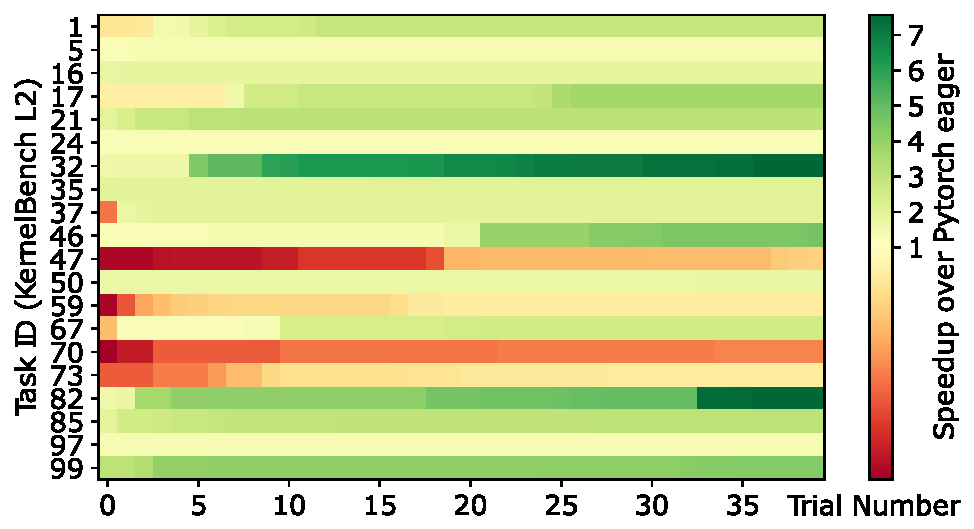
\includegraphics[width=0.6\linewidth]{Figures/heatmap_reduced_height.pdf}
    % \vspace{-6mm}
    \caption{Improvement over iterations (cumulative best)}
    \label{fig:speedup_iters}
    % \vspace{-5mm}
\end{figure}

\subsection{Validating hardware awareness}

To analyze whether our method produces hardware-aware kernels, we propose a crossover experiment: We run KernelFoundry on two distinctly different GPUs, here Intel Arc B580 and an integrated Intel Arc 140V GPU (LNL), and then benchmark the performance of the best generated kernels on the respective other GPU. If KernelFoundry is successful in generating hardware-aware kernels, we expect scenarios where the top-performing kernel of the LNL-run outperforms the best kernel optimized on B580 when both are benchmarked on LNL, 
and vice versa.
To quantify this, we introduce the hardware-speedup metric $hws$, defined as the speedup of a kernel $k^A$ optimized on GPU $A$ over a kernel $k_B$ optimized on GPU $B$: $hws(k^A) = \frac{t_{A} (k^B)}{t_A(k^A)}$, where $t_A$ is the runtime of a kernel on GPU $A$.  $hws_p$ is the percentage of kernels for which $hws > p $. We again use the representative subset of KernelBench L2 (20 tasks) and report average $hws$ for all kernels and $hws_p$ for $p$ equal to 1.0 and 1.5, i.e. the relative amount of kernels being quicker and 1.5 times quicker, respectively.  

\begin{table}[H]
\centering
\resizebox{0.6\linewidth}{!}{
    \begin{tabular}{lrrrr}
    \toprule
    Kernels & $hws_1$ & $hws_{1.5}$ & avg. hws & geom. hws \\
    \midrule
    LNL-optimized $k^{LNL}$ & 70 $\%$ & 20 $\%$ & 1.537 & 1.297 \\
    BMG-optimized $k^{B580}$  & 70  $\%$ & 15 $\%$ & 1.109 & 1.038 \\
    \bottomrule
    \end{tabular}
}
\caption{Evaluating hardware awareness. Kernels optimized for the target GPU outperform kernels optimized on another GPU.} 
\label{tab:hardware-aware}
% \vspace{-8mm}
\end{table}


As shown in \autoref{tab:hardware-aware}, 70\% of kernels are faster than their counterpart optimized on another GPU, with average speed-up of 1.537 for LNL-optimized kernels and 1.109 for BMG-optimized kernels. See Appendix~\ref{app:hardware} for per-task results.


\subsection{Beyond Pytorch Eager - comparison to oneDNN}
KernelBench and follow-ups usually just use Pytorch Eager and torch.compile as baselines, which is a good common ground but adds additional factors, like CPU overhead for routing to specific kernels of a backend library or the effectiveness of the compiled graph.
To eliminate these factors and demonstrate the flexibility of our framework beyond the KernelBench format, we directly compare to the high performance kernel library oneDNN.
We benchmark our framework on the operations shown in \autoref{tab:operations} implementing them with the C++ API of oneDNN and use operator fusion where possible.
For the \emph{concat(x, layernorm(x))} operation we use an initial implementation as starting point using our framework for kernel optimization. For the softmax operation we provide additional high level user guidance to implement an optimization idea that reduces the load on special function units inspired by Flash Attention 4. 
\autoref{tab:operations} shows that although the kernels in oneDNN are highly optimized, oftentimes implemented directly in assembly language, the generated SYCL kernels are competitive and provide a speedup in three cases. % For operations involving hardware acceleration for matrix multiplication which is not utilized in the generated kernels.
\begin{table}[h!]
    \centering
    \resizebox{0.7\linewidth}{!}{
    \begin{tabular}{lccc}
        \toprule
        \textbf{Operation} & \textbf{Initial impl.} & \textbf{User instructions} & \textbf{Speedup} \\
        \toprule
        concat(x, layer\_norm(x)) & X &  & 1.79 \\
        Matmul with relu post-op &  &  & 0.35 \\
        MaxPool + Linear &  &  & 0.72 \\
        Sum Reduction &  &  & 1.10 \\
        Softmax &  & X & 1.70 \\
        \bottomrule
    \end{tabular}
    }
    \caption{Speedup compared to the oneDNN C++ implementation}
    \label{tab:operations}
    % \vspace{-6mm}
\end{table}


\subsection{Case study: Accelerating an operation of Llama 3}
A common use case for kernel optimization is accelerating LMs on given hardware, often by allowing reduced precision as long as model performance is unaffected. As a case study, we target an operation in the Llama 3.2 1B model, the rotary positional embedding function, which presents a bottleneck on Intel hardware. We define a custom task (see \autoref{app:custom_task_infrastructure}) with the PyTorch implementation (\emph{apply\_rotary\_pos\_emb}, combining unsqueeze + rotate-half) as the reference. Correctness is tested by comparing our kernel’s output to the reference output, and by verifying that a full Llama3 model pass with our kernel yields identical results on a simple query. KernelFoundry discovers a correct kernel in just two iterations and achieves a 7.9× speedup within ten iterations. This accelerates the rotary embedding operation, resulting in an 8\% reduction in total forward pass time (from 0.413 s to 0.38 s) on a B580 Intel GPU.

